\chapter{System Methodology and CARLA\texorpdfstring{$\rightarrow$}{->}QLabs Adaptation}
\label{ch:methodology}

This chapter describes the system architecture and the concrete alignment steps required to run a SimLingo-style VLA driving policy in QLabs. The core idea is to treat simulator transfer as a \emph{systems alignment} problem: even when the model weights are identical, small mismatches in coordinate frames, timing, and measurement definitions can produce large closed-loop degradation.

\section{System architecture overview}
\label{sec:method-arch}
At runtime, the controller executes a closed-loop pipeline:
\begin{enumerate}[leftmargin=*]
  \item Capture the front camera image and ego-state (position/heading) from QLabs.
  \item Compute navigational conditioning (target points and optional high-level command).
  \item Construct a prompt and multimodal input batch.
  \item Run model inference to predict route waypoints and a speed profile.
  \item Convert model outputs into low-level QCar~2 controls via PID and rate limiting.
  \item Log trajectory, safety events, and diagnostics.
\end{enumerate}

This decomposition is reflected in the repository structure (\Cref{app:repo-map}): data collection is implemented under \path{data_collection/}, runtime control under \path{inference/}, and shared utilities under \path{core/}.

\section{Compatibility targets as distribution alignment}
\label{sec:compat-targets}
The guiding principle is \emph{distribution alignment}: the inference-time signals should match the training-time data format as closely as practical. In this repository the most important alignment targets are:
\begin{itemize}[leftmargin=*,itemsep=0.25em]
  \item \textbf{Coordinate frames:} target points and waypoints must be expressed in the same ego frame convention used during training.
  \item \textbf{Speed definition:} instantaneous speed should be computed in a way that matches the training data.
  \item \textbf{Prompt format:} the text prompt (including any placeholder tokens) must follow the pretrained template and training dataset conventions.
  \item \textbf{Sampling cadence:} differences in control frequency must be accounted for in PID conversion and in any finite-difference calculations.
\end{itemize}

\section{Key simulator differences}
\label{sec:sim-diffs}
\Cref{tab:carla-qlabs-diffs} summarizes simulator differences that directly influence implementation choices.

\begin{table}[h]
\centering
\caption{Implementation-relevant differences between CARLA and QLabs for this project.}
\label{tab:carla-qlabs-diffs}
\begin{tabular}{p{0.28\linewidth}p{0.30\linewidth}p{0.34\linewidth}}
\toprule
Category & CARLA (SimLingo context) & QLabs/QCar~2 adaptation\\
\midrule
Steering sign & Positive steer typically turns left & QCar~2 API uses opposite sign; steer must be negated in conversion (\Cref{ch:inference}).\\
Control cadence & Commonly \SI{20}{Hz} for control, data saved at \SI{4}{Hz} (every 5th frame) & Controller runs at \SI{4}{Hz}; derivative terms require frequency compensation.\\
Speed signal & Instantaneous velocity from simulator state & Estimated from single-frame displacement to match logged demonstrations.\\
Navigation conditioning & Target waypoint tokens and/or command text & Same conditioning reproduced by target points from routes + prompt construction.\\
Camera geometry & CARLA camera config & QLabs CSI camera FOV/resolution matched in config (\Cref{ch:inference}).\\
\bottomrule
\end{tabular}
\end{table}

Beyond these signal-level differences, the two simulators occupy fundamentally different points on the fidelity spectrum. CARLA is built on Unreal Engine~4 and provides photorealistic rendering (dynamic lighting, shadows, detailed road markings, diverse building textures), a full vehicle dynamics model (tire friction, inertia, suspension), and large, varied urban environments. QLabs, by contrast, is an educational platform with simplified rendering, a compact fixed-layout environment (\Cref{fig:sdcs-roadmap}), and an idealized vehicle model---for instance, the QCar~2 API accepts a commanded velocity that is applied without simulating braking inertia or traction limits. This fidelity gap has two competing implications for transfer. On one hand, visual features learned from CARLA's rich appearance distribution (e.g., shadow-aware lane detection, texture-based depth cues) may be underutilized or mismatched in QLabs' visually simpler scenes, potentially degrading perception performance. On the other hand, the simpler environment reduces visual clutter and dynamic variability, which can make the remaining signal-level alignment targets (coordinate frames, timing, speed estimation) the dominant factor in transfer quality---the premise on which the engineering work in this chapter is based. LoRA fine-tuning (\Cref{ch:training}) addresses the residual visual domain shift by adapting the model's visual and control grounding to QLabs imagery; the limitations of this approach are discussed further in \Cref{sec:limitations}.

\section{Coordinate frame alignment}
\label{sec:coord-align}
SimLingo training and inference operate primarily in the ego vehicle frame where $x$ points forward and $y$ points left. In this repository, the world\texorpdfstring{$\leftrightarrow$}{<->}ego conversion used for target points and route segments is implemented in \path{core/coordinate_utils.py}.

Let the ego pose in the world frame be a 2D translation $\mathbf{t}=[x_0,y_0]^\top$ and yaw (heading) $\psi$. For any world-frame point $\mathbf{p}_w=[x,y]^\top$, the corresponding ego-frame point is obtained by subtracting the ego translation and rotating into the ego heading:
\begin{equation}
\label{eq:world-to-ego}
\mathbf{p}_e = \mathbf{R}(-\psi)\left(\mathbf{p}_w-\mathbf{t}\right),\qquad
\mathbf{R}(\theta)=\begin{bmatrix}\cos\theta & -\sin\theta\\ \sin\theta & \cos\theta\end{bmatrix}.
\end{equation}
The inverse mapping is $\mathbf{p}_w=\mathbf{R}(\psi)\mathbf{p}_e+\mathbf{t}$. Keeping this convention consistent is critical because the model is trained on ego-frame route segments and target points; a sign or axis flip would systematically rotate or mirror the conditioning distribution.

\section{Target-point conditioning from routes}
\label{sec:target-point-conditioning}
QLabs scenarios specify an ego route as a sequence of world-frame waypoints (\Cref{app:scene-configs}). \Cref{fig:sdcs-roadmap} shows the QLabs SDCS environment layout with its numbered waypoint nodes. At runtime, the route manager implemented in \path{inference/route_manager.py} selects a lookahead target point along the polyline and converts it into the ego frame for prompt conditioning.

\begin{figure}[ht]
  \centering
  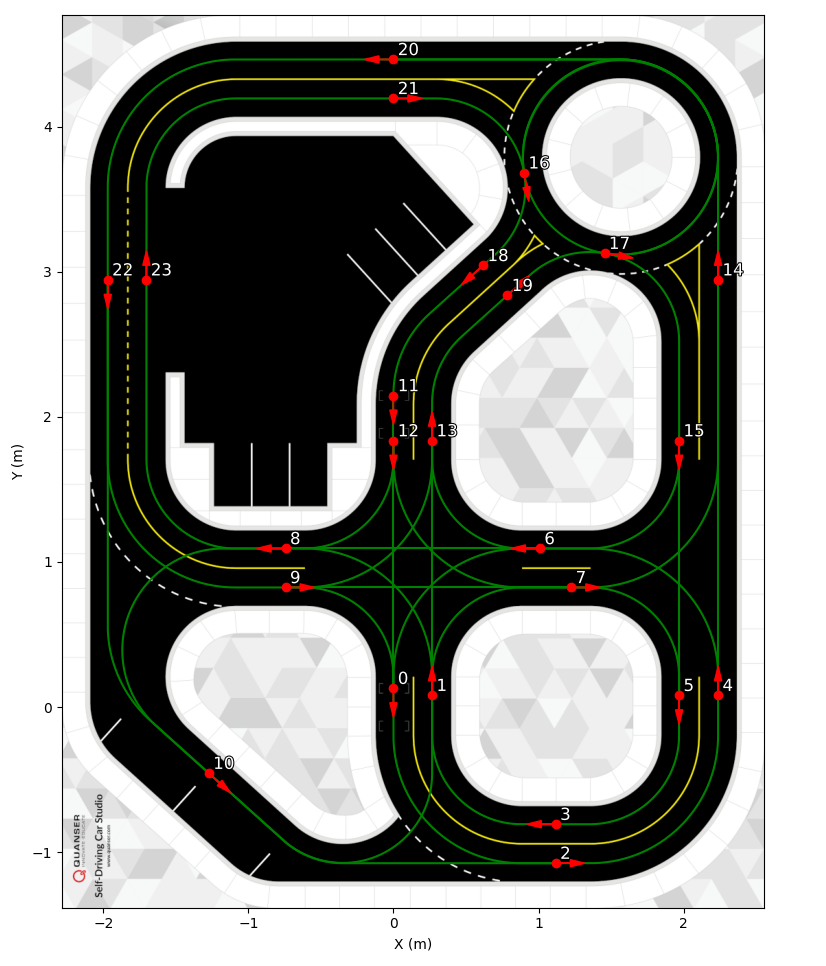
\includegraphics[width=0.85\textwidth]{figures/SDCS_RoadMap_RightHandTraffic.png}
  \caption{QLabs SDCS road map with numbered nodes representing waypoint locations. Routes are defined as ordered sequences of these nodes; the roundabout route used in this work traverses a subset of this layout.}
  \label{fig:sdcs-roadmap}
\end{figure}

Concretely, starting from the current (or nearest) route index $k$, the implementation advances along the waypoint list until the accumulated arc-length exceeds a configured lookahead distance $d$:
\begin{equation}
\label{eq:route-lookahead}
\text{find the smallest } j \ge k \text{ such that } \sum_{i=k}^{j-1}\lVert\mathbf{w}_{i+1}-\mathbf{w}_i\rVert_2 \ge d,\quad \mathbf{w}_i\in\mathbb{R}^2.
\end{equation}
The selected world-frame target $\mathbf{w}_j$ (and an optional ``next'' target farther ahead) are then mapped into the ego frame using \Cref{eq:world-to-ego}. Using target points rather than full route polylines matches SimLingo's target-point conditioning interface while keeping runtime computation lightweight.

\section{Traceability strategy}
\label{sec:traceability}
Throughout this thesis, design claims are tied to concrete source file paths in this repository (e.g., \path{inference/main.py}, \path{data_collection/data_recorder.py}). Rather than reproducing verbatim code, implementation details are described in prose and equations to keep the document readable while preserving technical specificity. Where hyperparameters are referenced, \Cref{app:hyperparameters} records the source YAML configuration files used for training and inference.
